\documentclass[11pt, a4paper]{article}
\usepackage{pdfpages}
\usepackage{parallel}
\usepackage[T2A]{fontenc}
\usepackage{ucs}
\usepackage[utf8x]{inputenc}
\usepackage[polish,english,russian]{babel}
\usepackage{hyperref}
\usepackage{rotating}
\usepackage[inner=2cm,top=1.8cm,outer=2cm,bottom=2.3cm,nohead]{geometry}
\usepackage{listings}
\usepackage{graphicx}
\usepackage{wrapfig}
\usepackage{longtable}
\usepackage{indentfirst}
\usepackage{array}
\usepackage{tikzsymbols}
\usepackage{soul}
\usepackage[ruled,vlined]{algorithm2e}
%\counterwithout{figure}{section} 

\usepackage{url}
\makeatletter
\g@addto@macro{\UrlBreaks}{\UrlOrds}
\makeatother

\newcolumntype{P}[1]{>{\raggedright\arraybackslash}p{#1}}
\frenchspacing
\usepackage{fixltx2e} %text sub- and superscripts
\usepackage{icomma} % коскі ў матэматычным рэжыме
\PreloadUnicodePage{4}

\newcommand{\longpage}{\enlargethispage{\baselineskip}}
\newcommand{\shortpage}{\enlargethispage{-\baselineskip}}

\def\switchlang#1{\expandafter\csname switchlang#1\endcsname}
\def\switchlangbe{
\let\saverefname=\refname%
\def\refname{Літаратура}%
\def\figurename{Іл.}%
}
\def\switchlangen{
\let\saverefname=\refname%
\def\refname{References}%
\def\figurename{Fig.}%
}
\def\switchlangru{
\let\saverefname=\refname%
\let\savefigurename=\figurename%
\def\refname{Литература}%
\def\figurename{Рис.}%
}

\hyphenation{admi-ni-stra-tive}
\hyphenation{ex-pe-ri-ence}
\hyphenation{fle-xi-bi-li-ty}
\hyphenation{Py-thon}
\hyphenation{ma-the-ma-ti-cal}
\hyphenation{re-ported}
\hyphenation{imp-le-menta-tions}
\hyphenation{pro-vides}
\hyphenation{en-gi-neering}
\hyphenation{com-pa-ti-bi-li-ty}
\hyphenation{im-pos-sible}
\hyphenation{desk-top}
\hyphenation{elec-tro-nic}
\hyphenation{com-pa-ny}
\hyphenation{de-ve-lop-ment}
\hyphenation{de-ve-loping}
\hyphenation{de-ve-lop}
\hyphenation{da-ta-ba-se}
\hyphenation{plat-forms}
\hyphenation{or-ga-ni-za-tion}
\hyphenation{pro-gramming}
\hyphenation{in-stru-ments}
\hyphenation{Li-nux}
\hyphenation{sour-ce}
\hyphenation{en-vi-ron-ment}
\hyphenation{Te-le-pathy}
\hyphenation{Li-nux-ov-ka}
\hyphenation{Open-BSD}
\hyphenation{Free-BSD}
\hyphenation{men-ti-on-ed}
\hyphenation{app-li-ca-tion}

\def\progref!#1!{\texttt{#1}}
\renewcommand{\arraystretch}{2} %Іначай формулы ў матрыцы зліпаюцца з лініямі
\usepackage{array}

\def\interview #1 (#2), #3, #4, #5\par{

\section[#1, #3, #4]{#1 -- #3, #4}
\def\qname{LVEE}
\def\aname{#1}
\def\q ##1\par{{\noindent \bf \qname: ##1 }\par}
\def\a{{\noindent \bf \aname: } \def\qname{L}\def\aname{#2}}
}

\def\interview* #1 (#2), #3, #4, #5\par{

\section*{#1\\{\small\rm #3, #4. #5}}
\ifx\ParallelWhichBox\undefined%
    \addcontentsline{toc}{section}{#1, #3, #4}%
\else%
\ifnum\ParallelWhichBox=0%
    \addcontentsline{toc}{section}{#1, #3, #4}%
\fi\fi%

\def\qname{LVEE}
\def\aname{#1}
\def\q ##1\par{{\noindent \bf \qname: ##1 }\par}
\def\a{{\noindent \bf \aname: } \def\qname{L}\def\aname{#2}}
}

\newcommand{\interviewfooter}[1]{
\vskip 1em
\noindent \textit{#1}
}

\switchlang{en}
\begin{document}

\title{1992 "--- IBM PS/2 Track Ball, a trackball/mouse combo}
\date{}
\maketitle
\selectlanguage{english}
In 1992, IBM released a non-standard flip trackball that could work in two modes: a trackball (figure \ref{fig:IBMConvertibleTrackball}) and a regular mouse (\ref{fig:IBMConvertibleMouse}).

\begin{figure}[h]
    \centering
    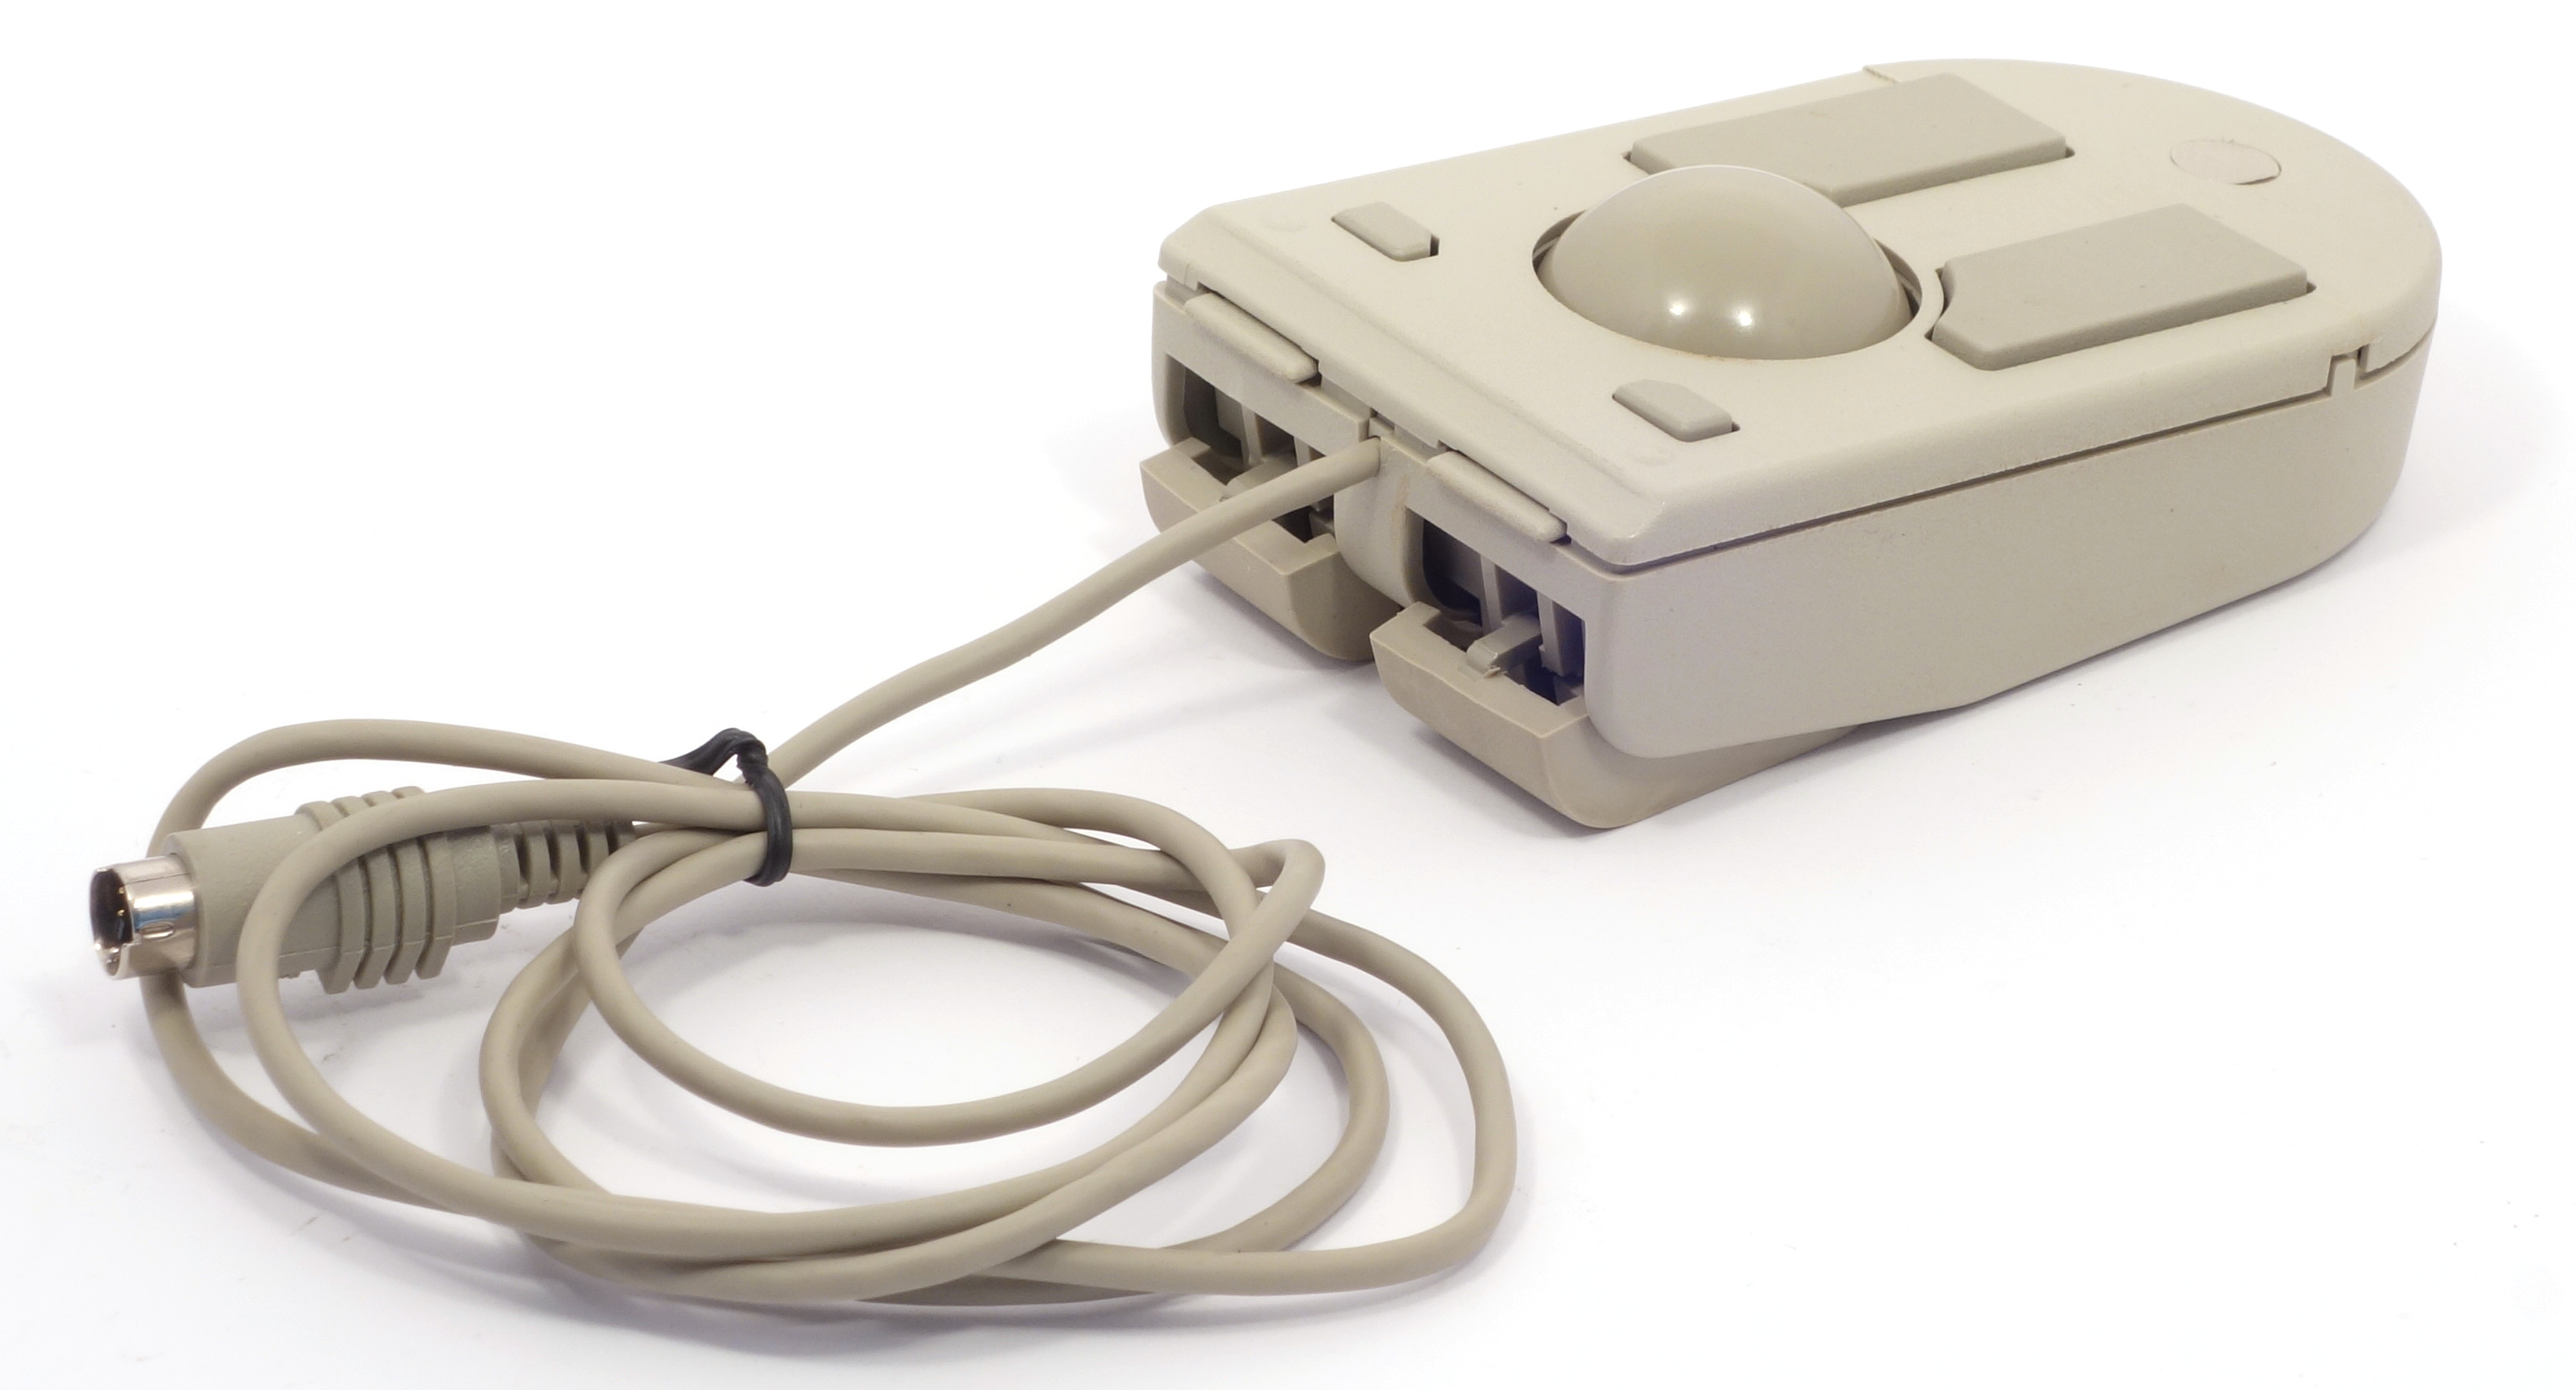
\includegraphics[scale=0.5]{1992_ibm_convertible/picball_60}
    \caption{IBM PS/2 Track Ball, trackbal mode}
    \label{fig:IBMConvertibleTrackball}
\end{figure}

\begin{figure}[h]
    \centering
    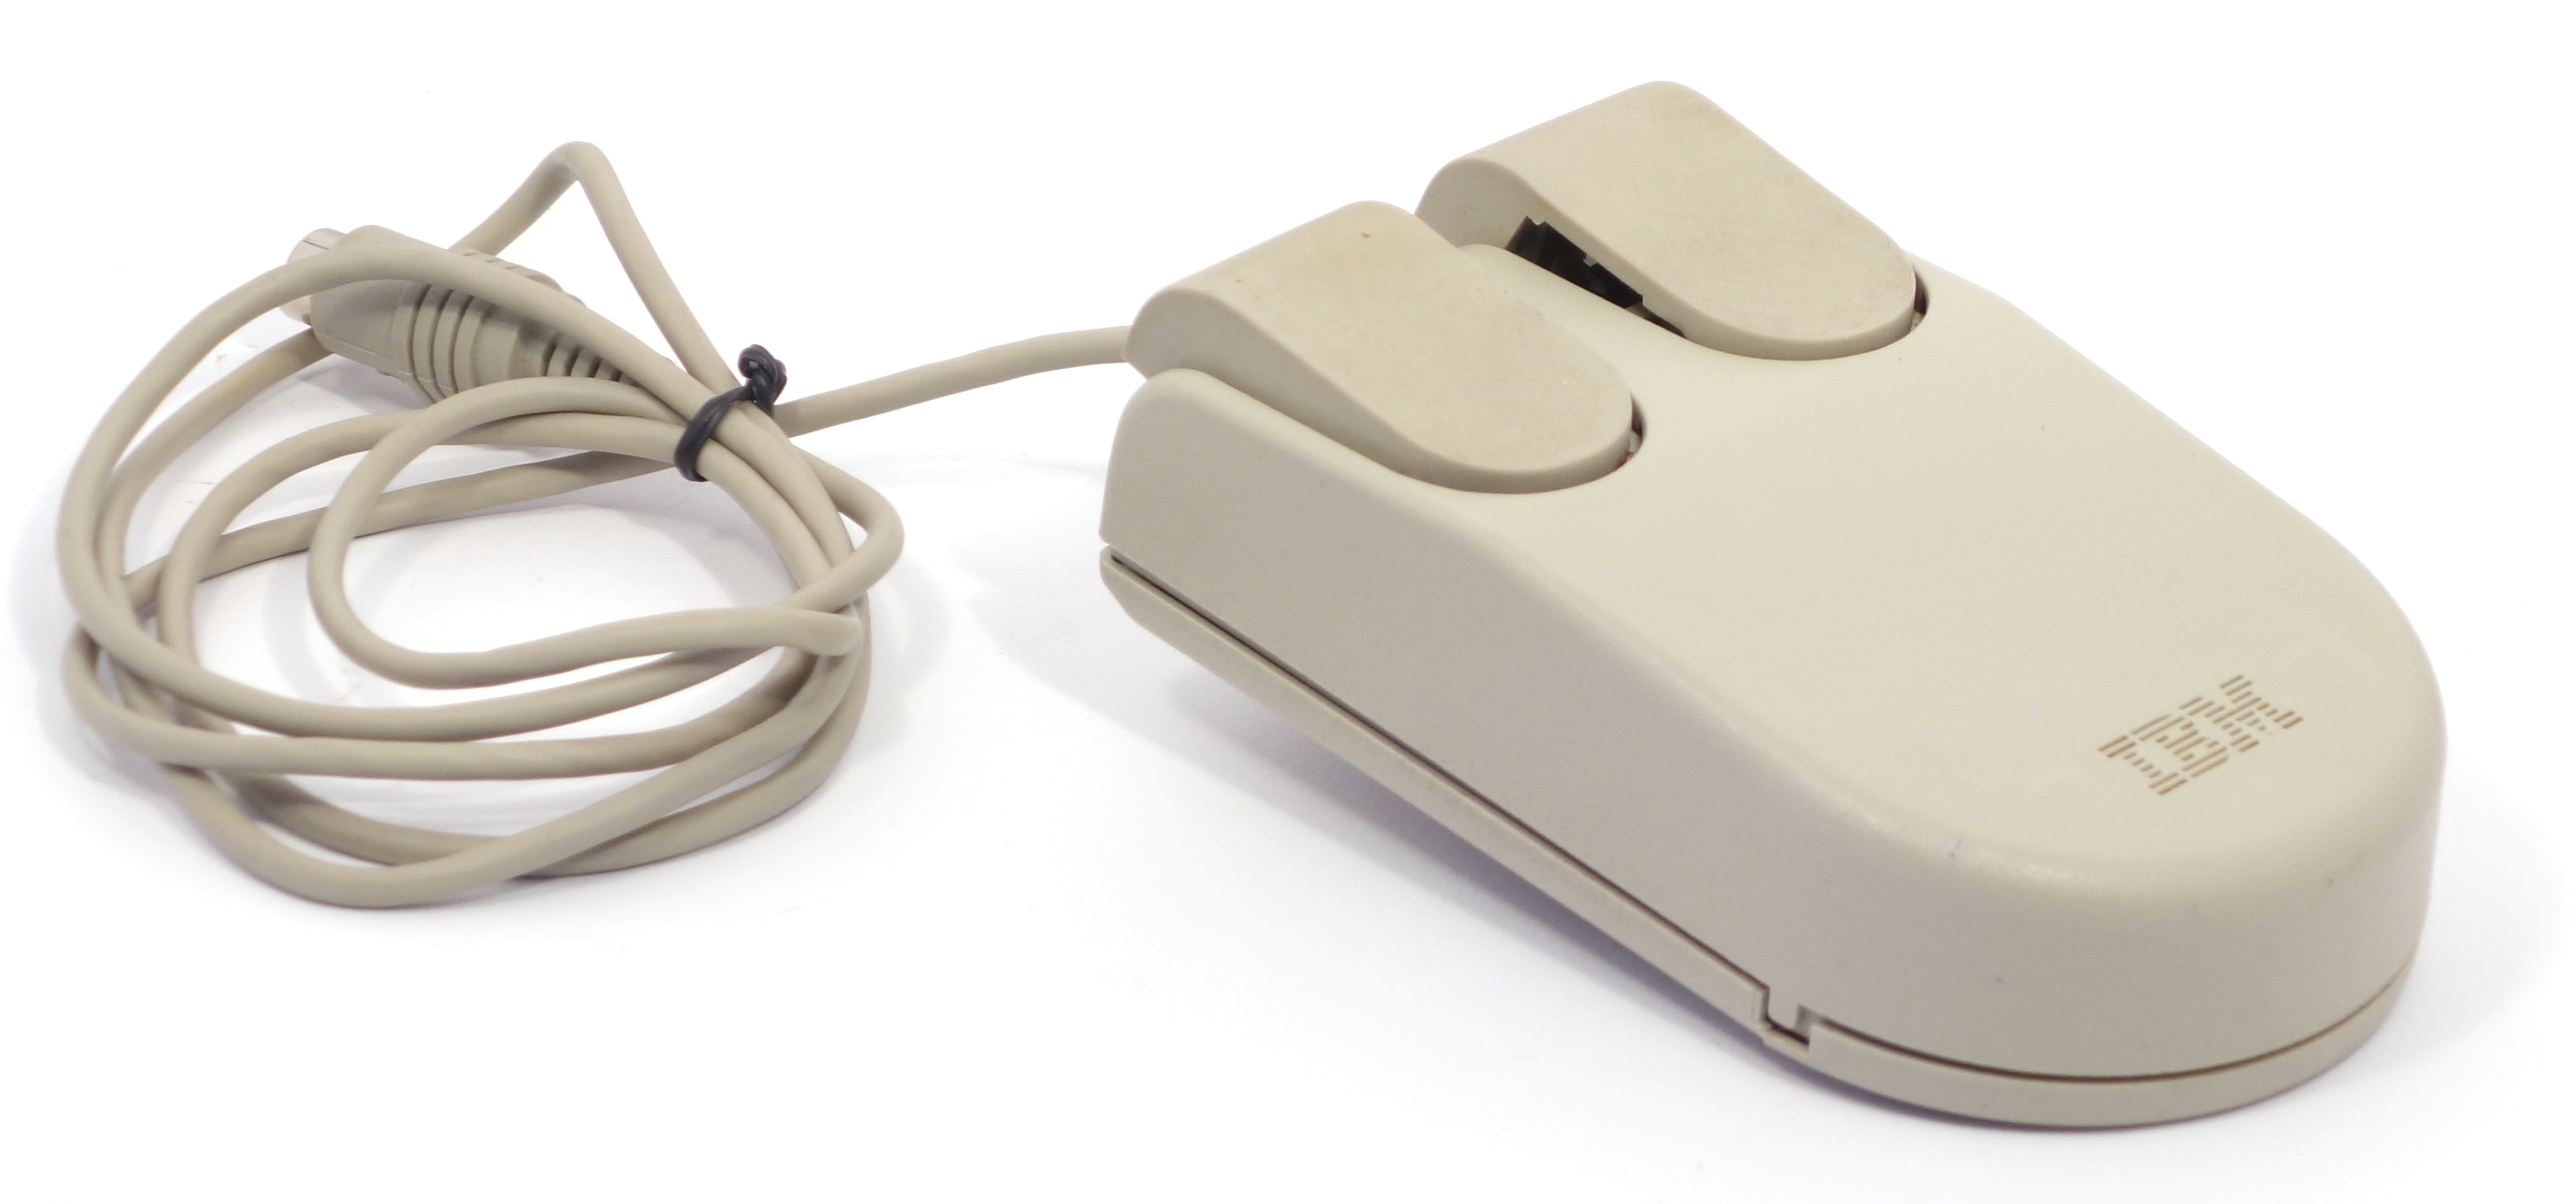
\includegraphics[scale=0.5]{1992_ibm_convertible/picmouse_60}
    \caption{IBM PS/2 Track Ball, mouse mode}
    \label{fig:IBMConvertibleMouse}
\end{figure}

Converting the device from one mode to another is performed by pressing a pair of plastic latches that change the position of the upper - or, depending on the mode of operation, the lower - side of the case. As a result, the ball and the buttons located next to it protrude more or less from the body \cite{mouses}.

\begin{figure}[h]
    \centering
    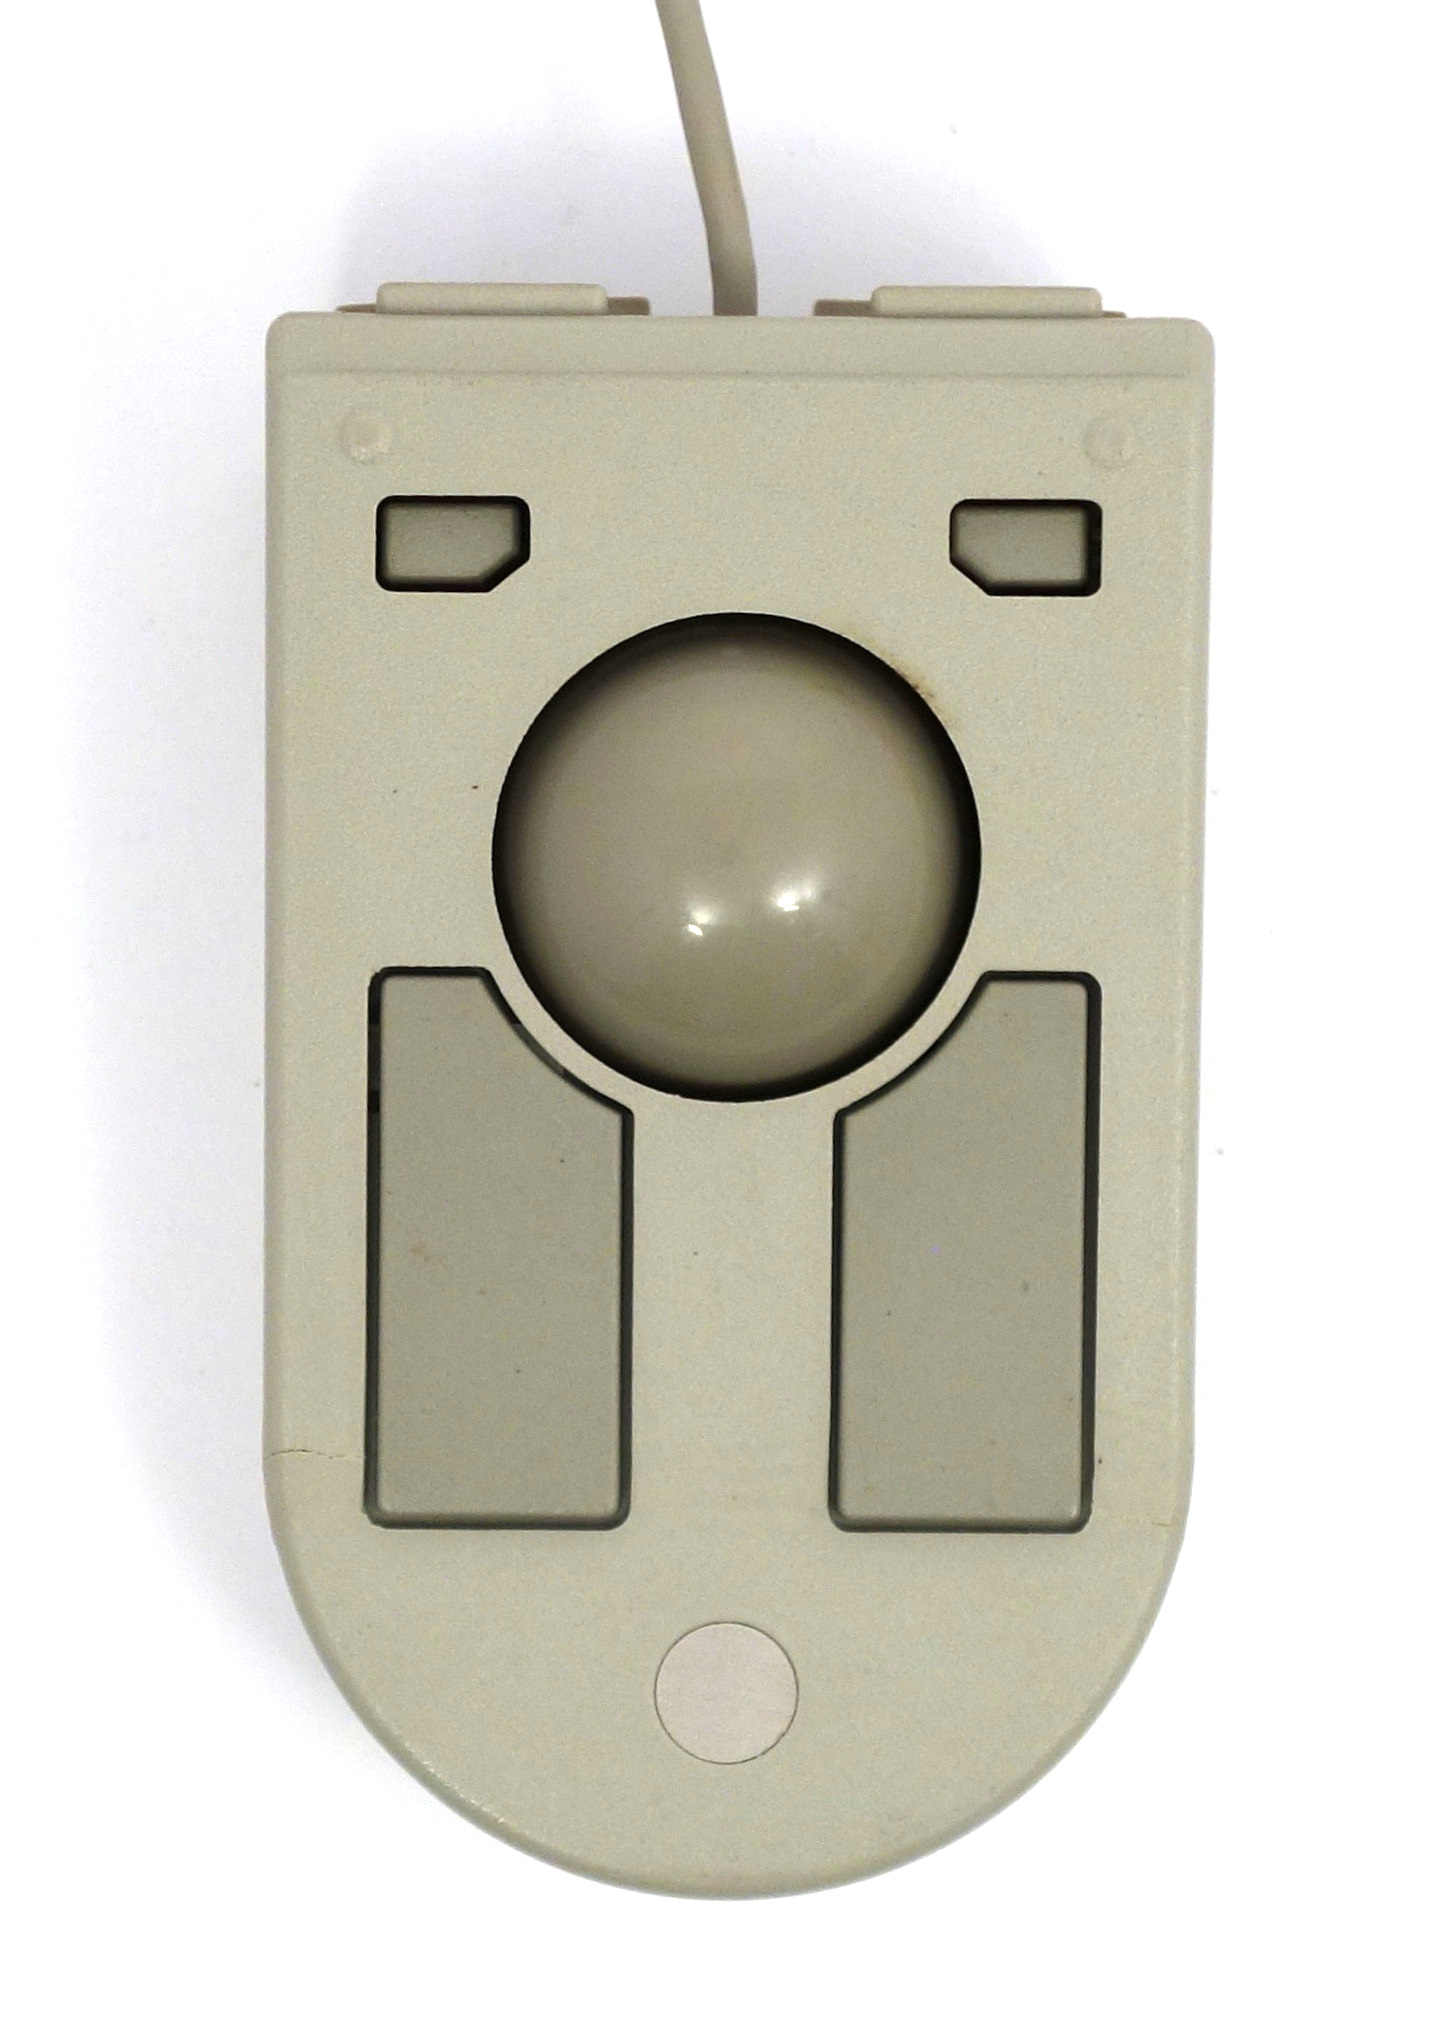
\includegraphics[scale=0.56]{1992_ibm_convertible/top_60.jpg}
    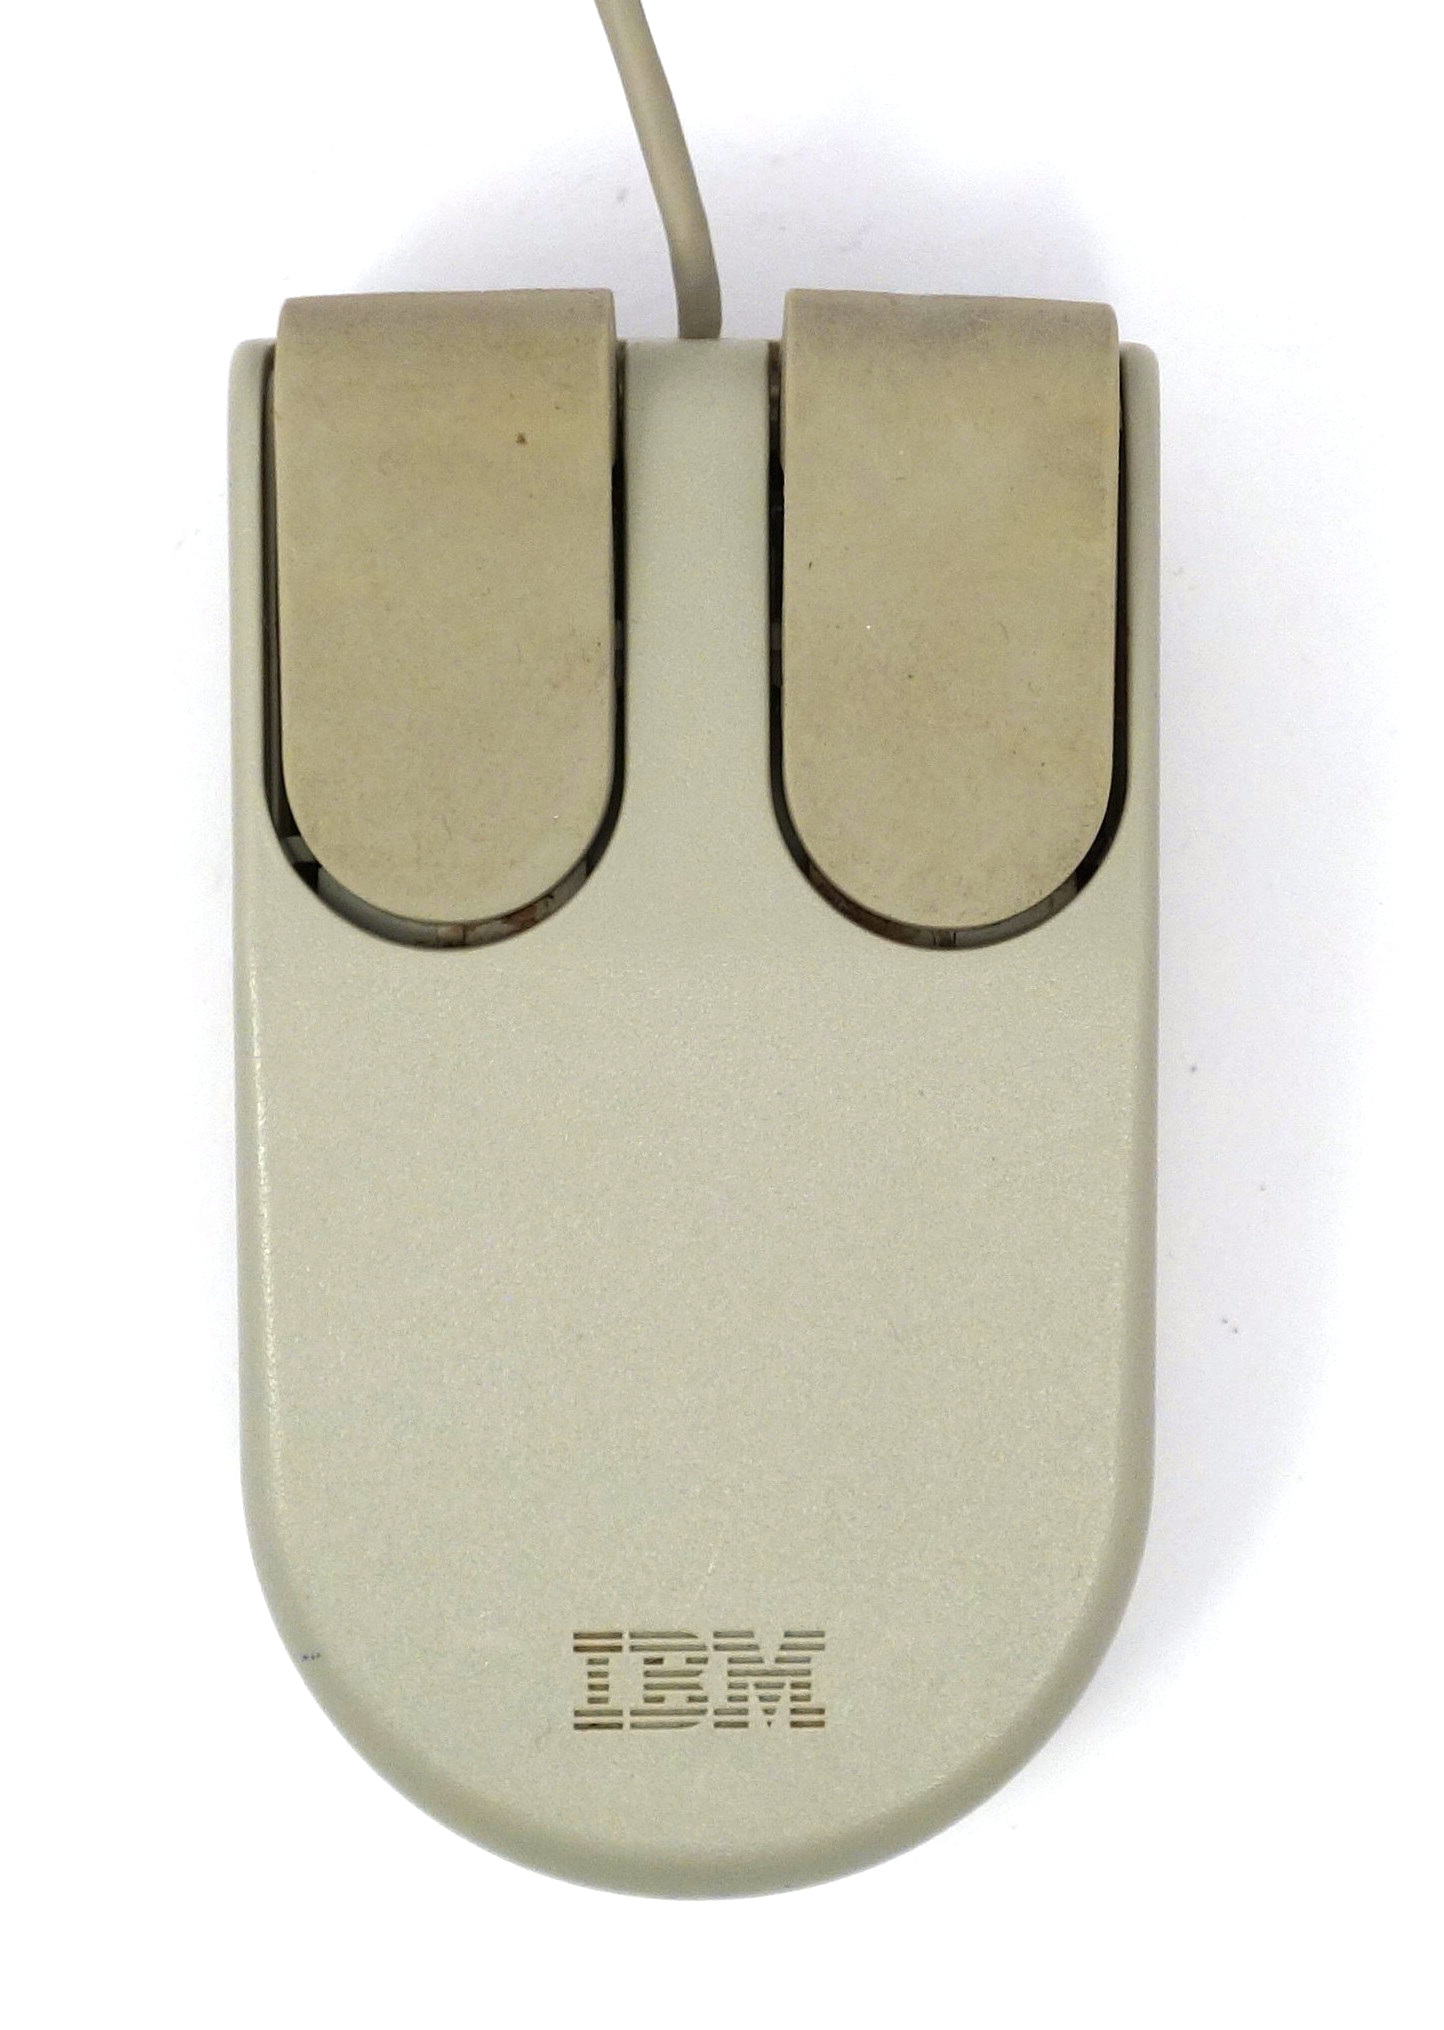
\includegraphics[scale=0.56]{1992_ibm_convertible/bottom_60.jpg}
    \caption{IBM PS/2 Track Ball views: trackball view (left), mouse view (right)}
    \label{fig:IBMConvertibleTopAndBottom}
\end{figure}

There are 4 keys on the trackball side of the device (figure \ref{fig:IBMConvertibleTopAndBottom}): 2 large keys are the left and right mouse buttons, respectively, 2 small buttons are latches, and pressing them blocks the keys on the opposite side of the device. On the mouse side, there is the IBM logo and two large buttons. The device itself is compact, suitable for portable use (figure \ref{fig:IBMConvertibleSize}).

\begin{figure}[h]
    \centering
    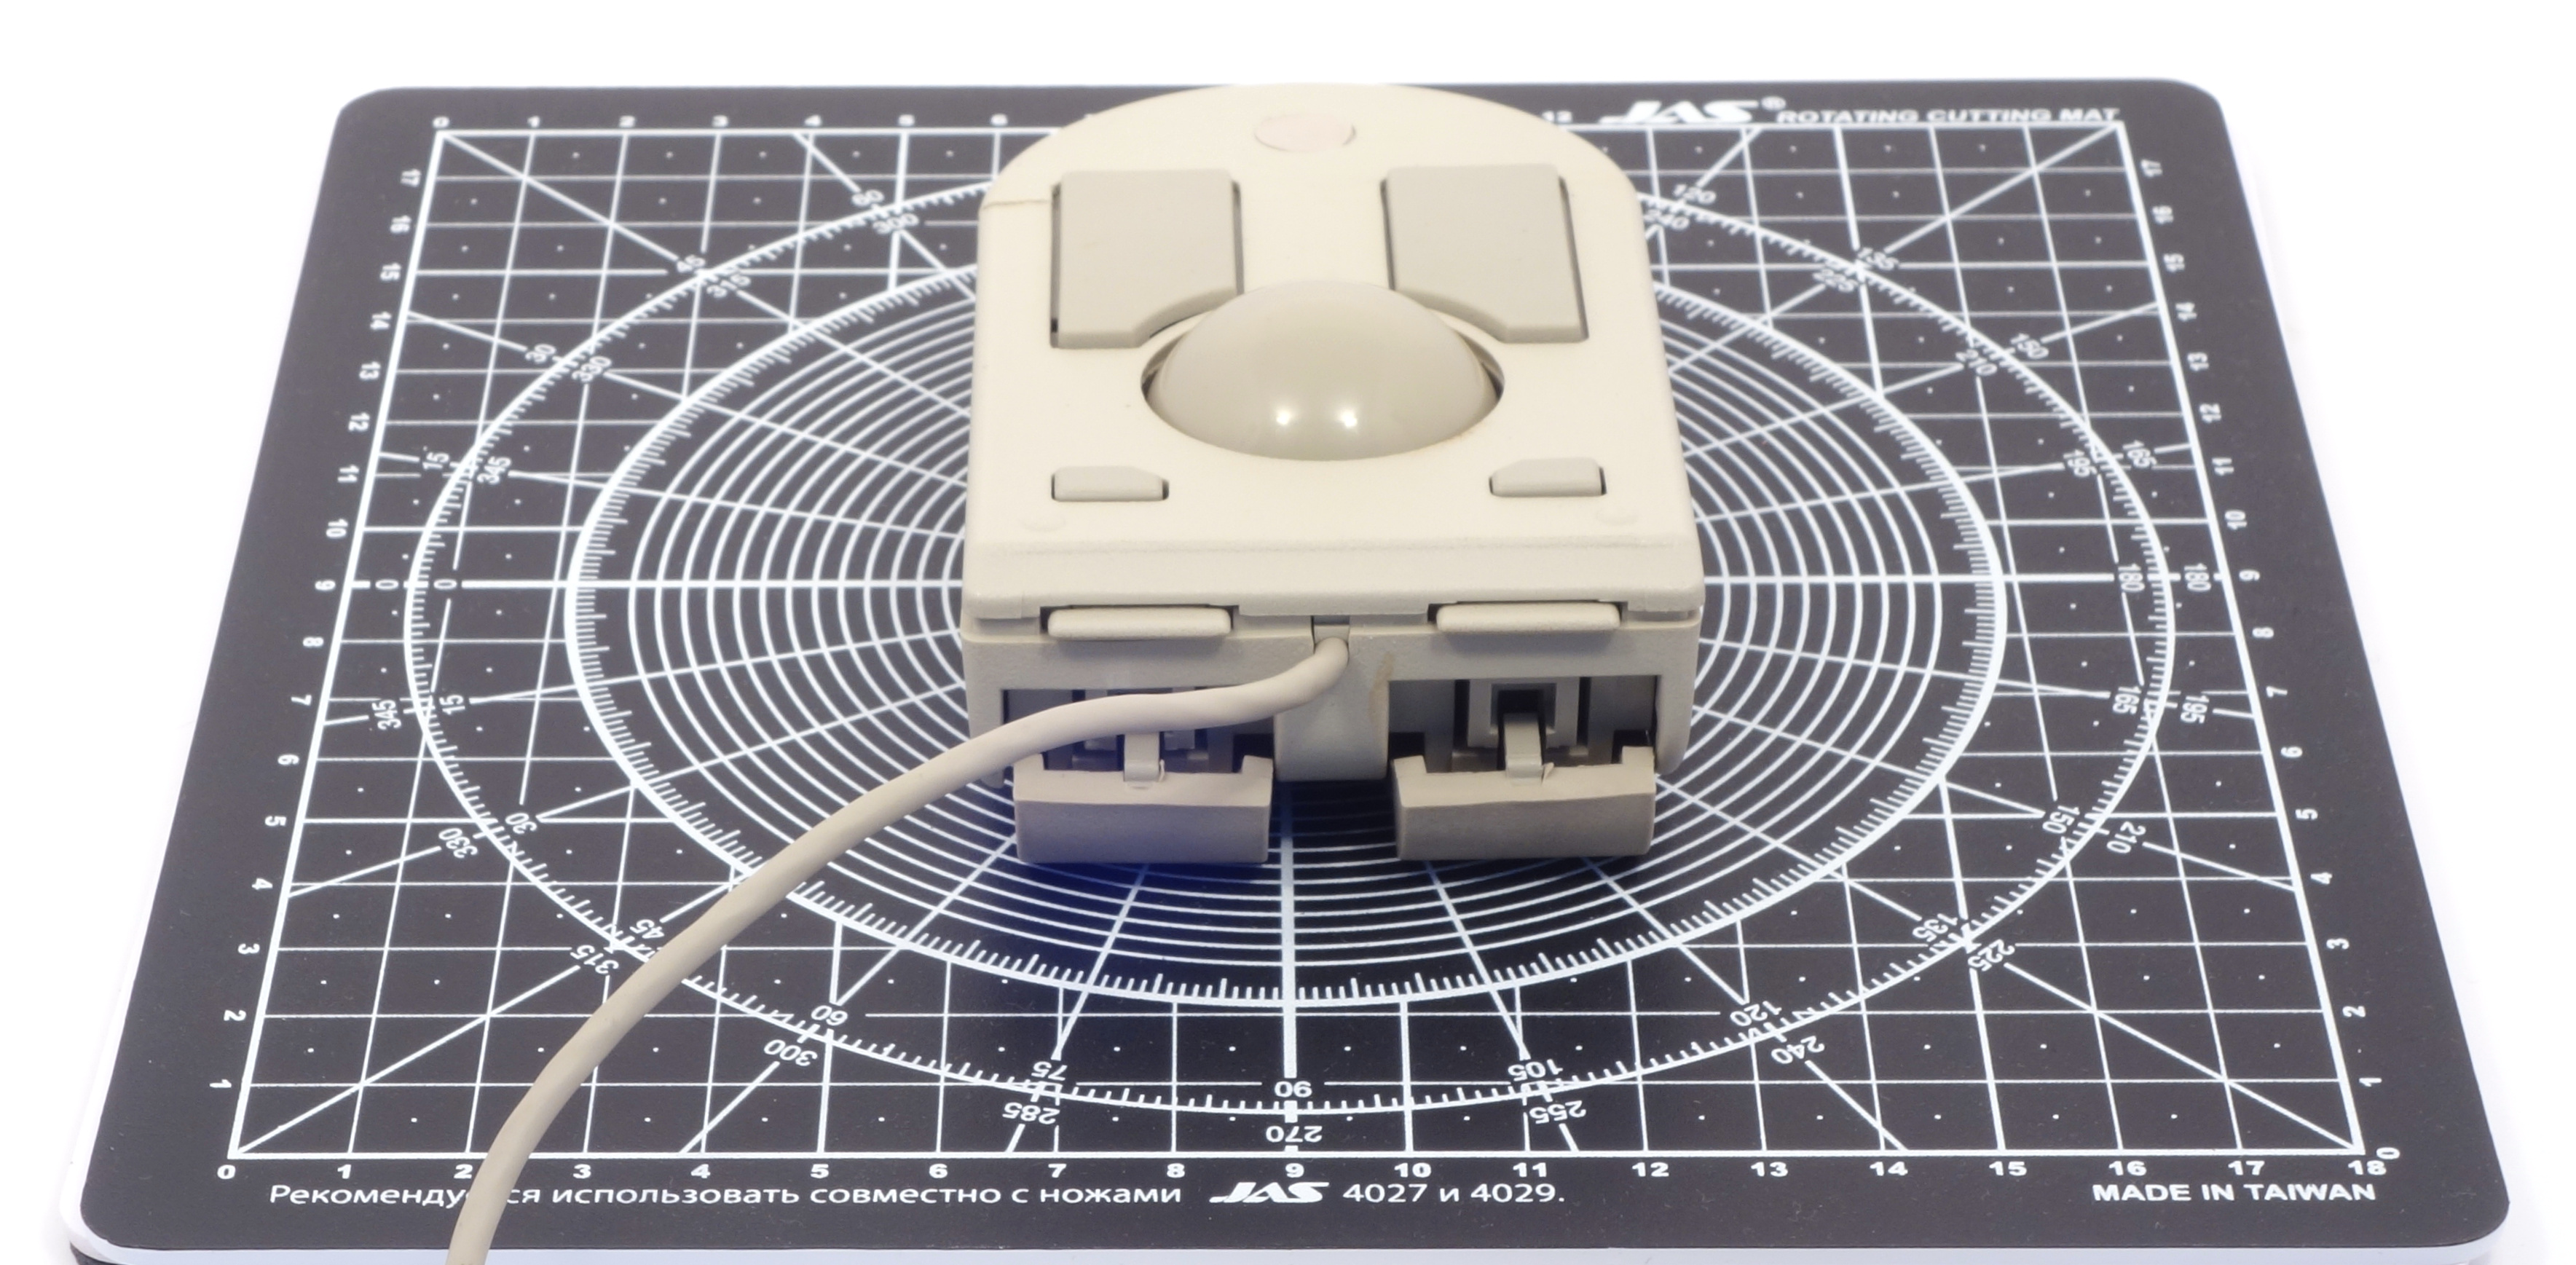
\includegraphics[scale=0.56]{1992_ibm_convertible/size_30.jpg}
    \caption{BM PS/2 Track Ball on a graduated pad with a grid step of 1~cm}
    \label{fig:IBMConvertibleSize}
\end{figure}

Given the anatomical structure of the hand, the device has a fairly ergonomic shape, and large keys are comfortable to press with fingers (figure \ref{fig:IBMConvertibleHand}). However, it is difficult to use the manipulator as a mouse on many surfaces due to the smoothness of the ball. It also turns out to be problematic to use it as a trackball, since in this mode the device stands on two protruding mouse buttons, which negatively affects its stability \cite{IBM}.

\begin{figure}[h]
    \centering
    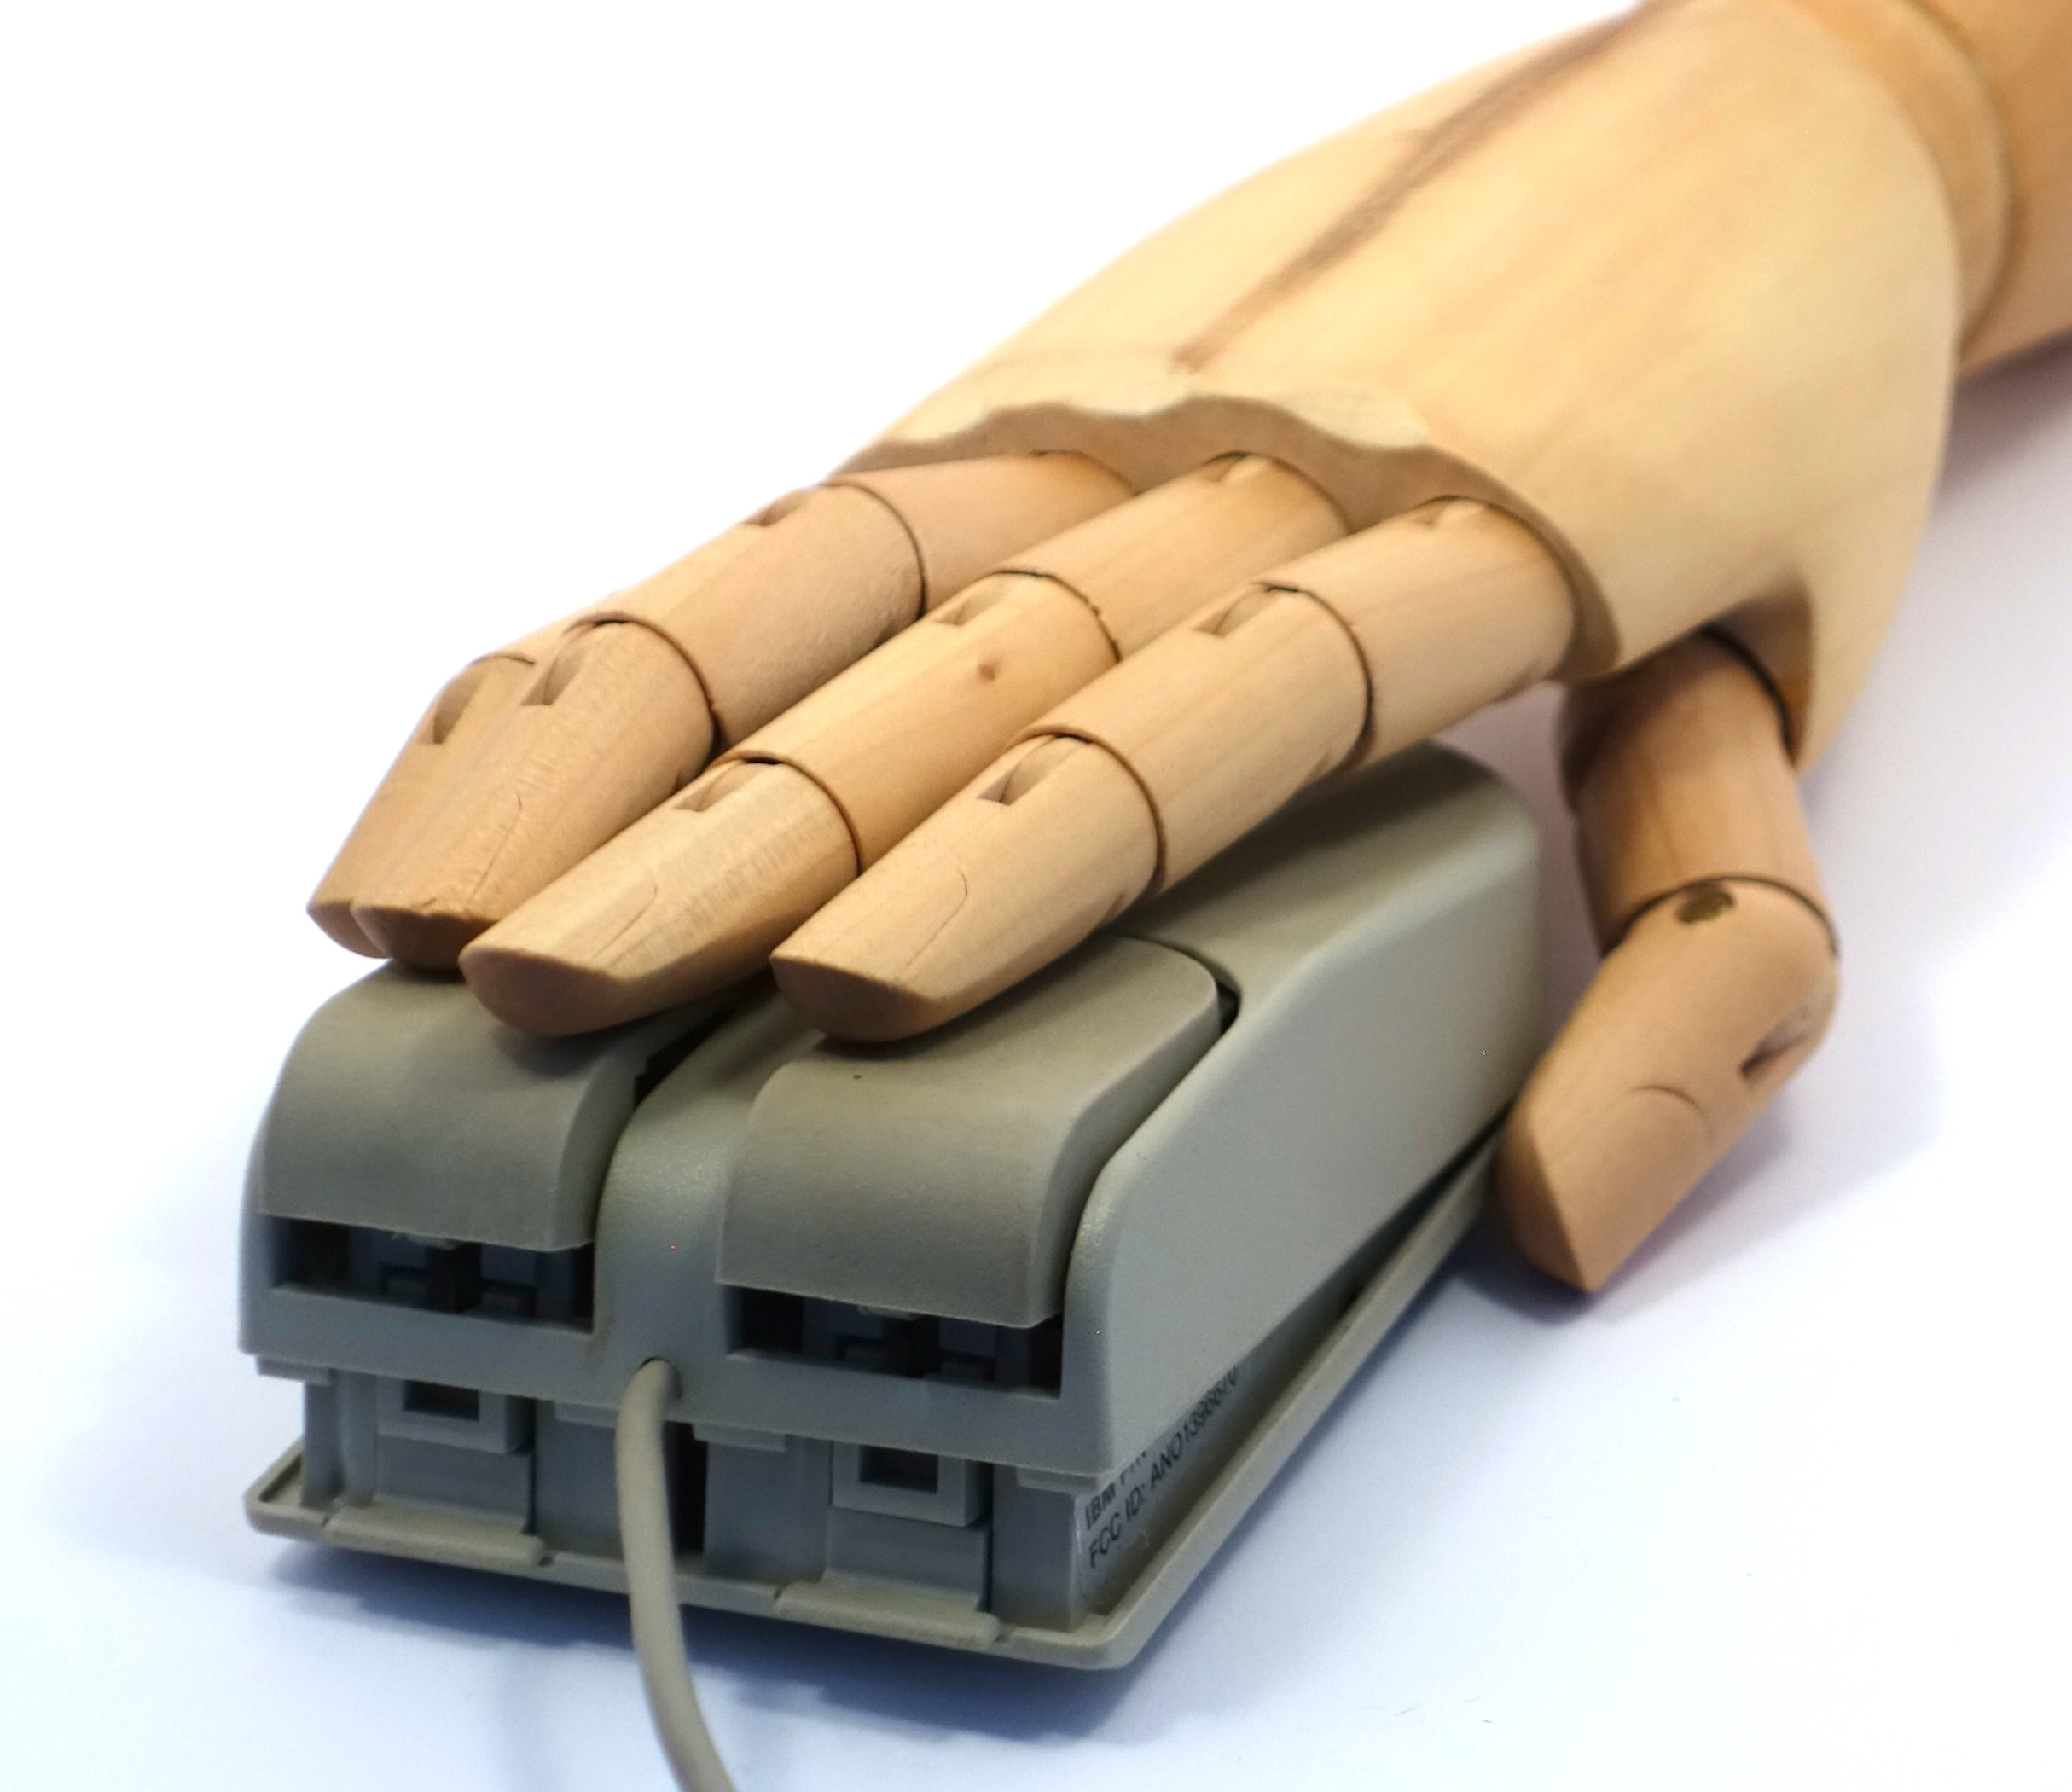
\includegraphics[scale=0.45]{1992_ibm_convertible/hand_60.jpg}
    \caption{IBM PS/2 Track Ball with a human hand model}
    \label{fig:IBMConvertibleHand}
\end{figure}

Trackball internals are shown on figure (\ref{fig:IBMConvertibleInside}). The standard opto-mechanical design is supplemented by massive metal rollers with rolling bearings. Standard PS/2 port was used for connecting this mouse to PC.

\begin{figure}[h]
    \centering
    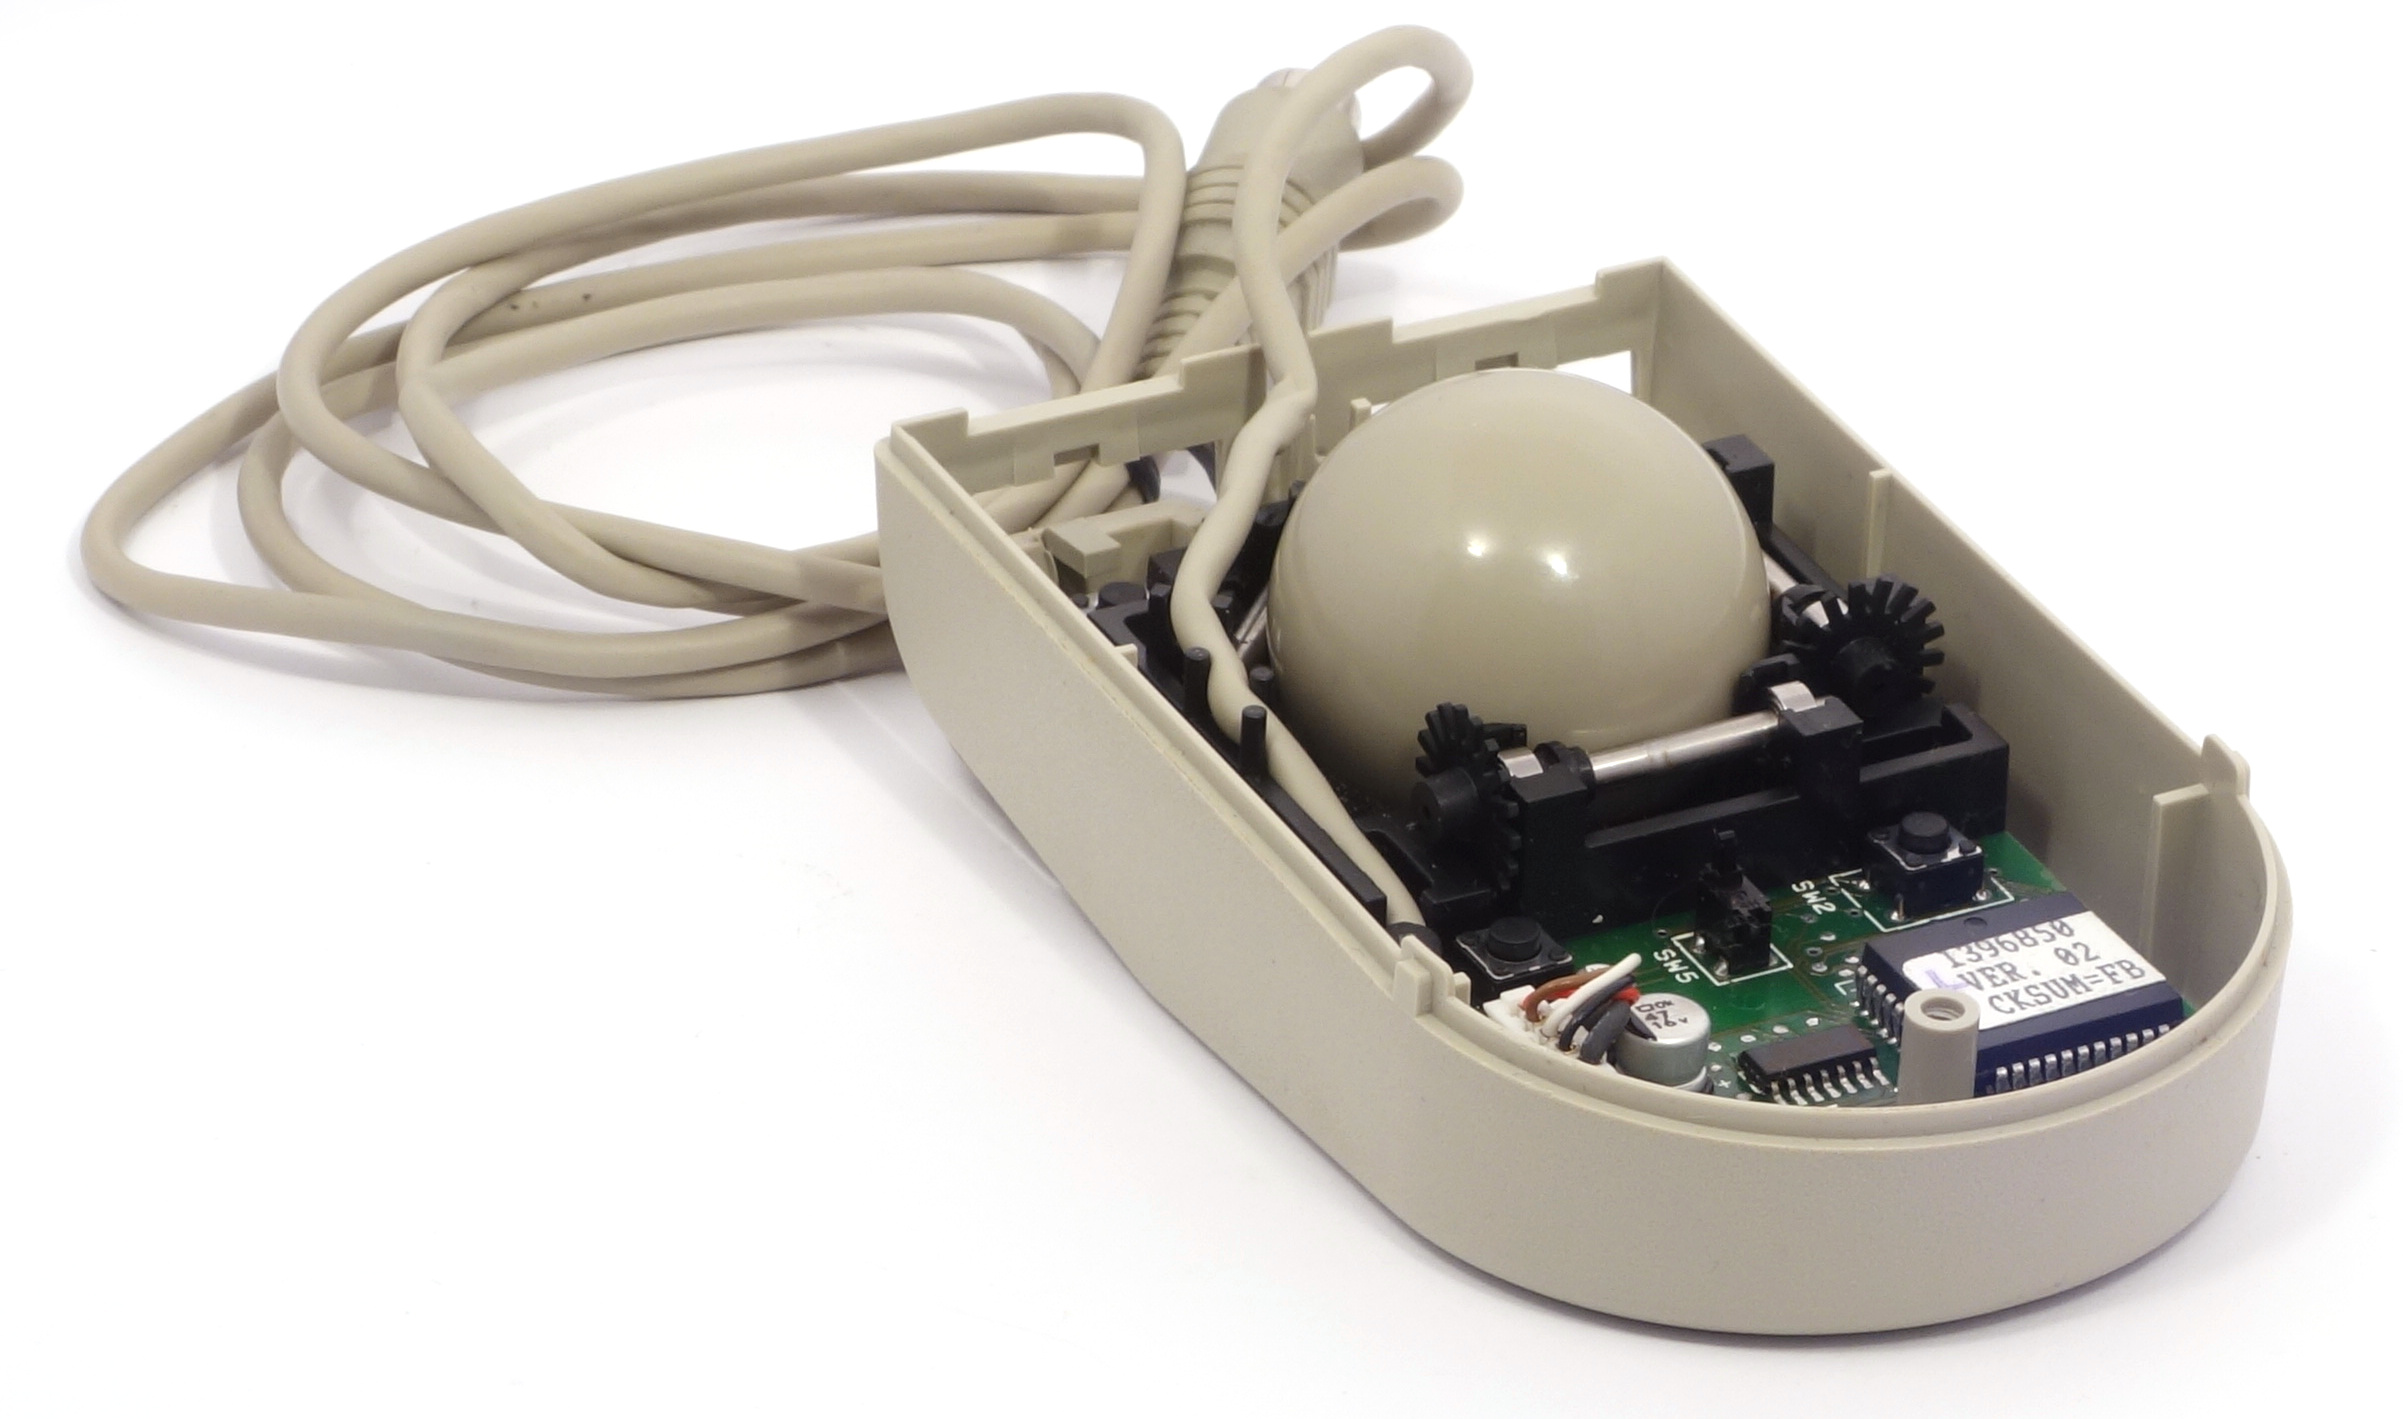
\includegraphics[scale=0.7]{1992_ibm_convertible/inside_60.jpg}
    \caption{BM PS/2 Track Ball disassembled}
    \label{fig:IBMConvertibleInside}
\end{figure}

The design does not provide for a way to open trackball for cleaning, with the exception of peeling off a round plug, which closes the fastener screw (it can be seen on the lef part of the Figure \ref{fig:IBMConvertibleTopAndBottom}). Considering that small garbage inevitably gets into the body of mechanical mice and trackballs, the question of the long-term operation of this device complements its controversial ergonomic characteristics.

~

~

\begin{thebibliography}{9}
\bibitem {mouses} Quain J.R. IBM PS/2 trackpoint // PC Magazine. October 15, 1991. p. 126 \url{https://books.google.by/books?id=tSLe3yMjc-AC&lpg=PP1&pg=PT123#v=onepage&q&f=false}
\bibitem {IBM} IBM PS/2 L40SX "Convertible" Pointing Device \url{https://www.youtube.com/watch?v=-OSXeNVM3UI&ab_channel=uxwbill}
\end{thebibliography}
\end{document}
